\documentclass[Softwaredesign/Softwaredesign_main.tex]{subfiles}
\begin{document}
\subsection{Klassediagram}
\begin{figure}
    \centering
    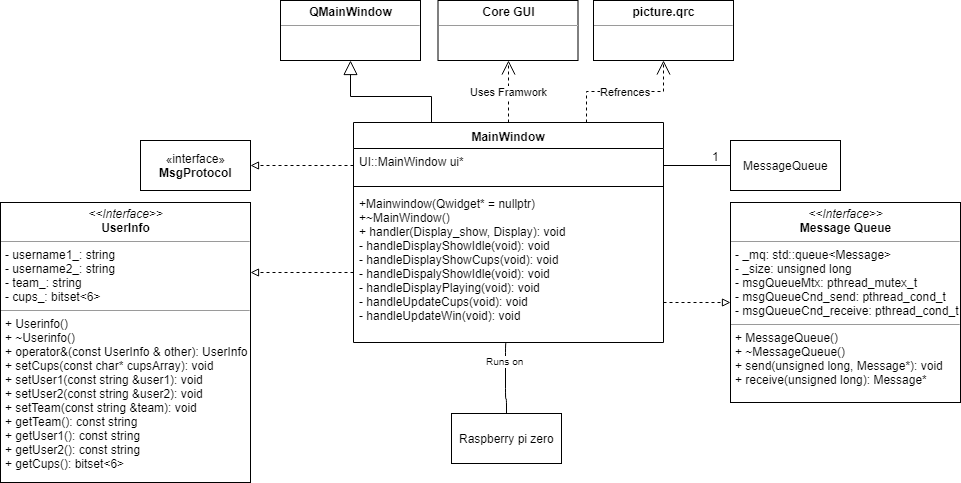
\includegraphics[scale=0.4]{Softwaredesign/GUI/Pictures/Guiklassediagram.png}
    \caption{Klasse diagram for relevante: Klasser, interfaces, Enums, Frameworks og ressourcer, som bliver brugt sammen med MainWindow klassen}
    \label{fig:Gui_klassediagram}
\end{figure}

På figur \ref{fig:Gui_klassediagram} ses der et klasse diagram, med relevante forbindelser til MainwWindow klassen, som er "hoved" klassen for GUI. 

\subsubsection{Framework}
Hele GUI systemet er baseret på "Core GUI" (se figur \ref{fig:Gui_klassediagram}), som et QT creator framework. Dette framework benyttes da det er crossplatform kompatibel: Linux, Windows, MacOS. Det giver også en grafisk interface at designe GUI'en med, hvilket reducere udviklings tiden substantielt. 

\subsubsection{Ressourcer}
Der der benyttes ordinære "PNG" format billeder, skal de lagres et sted sammen mea applikationen. QT frameworket gør det muligt at lave en ".qrc" ressource fil; ressource filer bindes bindes til mapper via. præfiks. Så til en billede ressource kan man have en "billede.qrc", som har en f.eks. et "logo" præfiks som er bundet til en "logo" mappe som indeholder billeder af logoer. I dette tilfælde som det ses på figur \ref{fig:Gui_klassediagram}, er der en "picture" ressource, som kan reffere til en mappe med billeder gennem "pic" præfikset. Dette gør at stien til brugte billeder er statiske, og ikke ændre sig fra system til system, men derimod gemmes hos applicationen.

\subsubsection{MsgProtocol}
På figur \ref{fig:Gui_klassediagram} kan der ses en MsgProtocol (kort for Message protocol). Detter er simpelt bare en liste over Enums, som svare til forskellige beskeder ,som kan sendes over en givet MessageQueue. 

\subsubsection{Message Queue}
På figur \ref{fig:Gui_klassediagram} kan der både ses et MessageQueue object, samt en Message Queue interface. Dette er tilfældet da der altid istantierer et MessageQueue objekt, ved program start; for at kunne kommunikere med den MessageQueue skal Message Queue interfacen bruges. For eksempel hvis der skal trækkes et objekt ud af MessageQueue, skal der bruges en get metode fra Message Queue interface. 

\subsubsection{Userinfo}
På figur \ref{fig:Gui_klassediagram} ser en Userinfo interface. Dette interface bruges for dets get funktioner; da MainWindow ikke selv har noget logik i sig, så skal den bruge en grænseflade til at få adgang til information omkring spillets status. Så hvis "update cups" bliver kaldt, skal klassen vide hvad status for hver enkelt cup er, så der i det tilfælde skal den bruge "getCups" funktionen. 



\end{document}